\documentclass[11pt]{article}

\usepackage[margin=1in]{geometry}
\usepackage{booktabs}
\usepackage{caption}
\usepackage{float}
\usepackage{graphicx}
\usepackage{hyperref}
\usepackage{longtable}
\usepackage{microtype}
\usepackage{amsmath}
\usepackage{array}

\captionsetup{font=small,skip=4pt}
\setlength{\textfloatsep}{8pt plus 2pt minus 2pt}
\setlength{\floatsep}{8pt plus 2pt minus 2pt}
\setlength{\intextsep}{8pt plus 2pt minus 2pt}
\renewcommand{\topfraction}{0.92}
\renewcommand{\bottomfraction}{0.82}
\renewcommand{\textfraction}{0.08}
\renewcommand{\floatpagefraction}{0.78}
\setcounter{topnumber}{3}
\setcounter{bottomnumber}{2}
\setcounter{totalnumber}{5}

\hypersetup{
  colorlinks=true,
  linkcolor=black,
  citecolor=black,
  urlcolor=blue
}

\title{Organizational Authenticity and Corporate Value Alignment:\\
A Scalable Text-Based Measurement Pipeline}
\author{}
\date{\today}

\begin{document}
\maketitle

\begin{abstract}
This measurement pipeline develops and validates a reproducible text-based approach for studying
organizational authenticity as alignment between firms' stated values and priorities reflected in
official disclosures. In a fixed sample of 50 large S\&P 500 firms across Technology, Financials,
Healthcare, Consumer Discretionary, and Energy from 2016--2024, I collect archived corporate
stated-values pages from the Wayback Machine, pair them with SEC definitive proxy statements
(\texttt{DEF 14A}), and construct an Organizational Authenticity Index from overlap between
12-theme distributions. The panel retains all 450 target company-years, including 358 usable
stated-values observations, 434 collected proxy statements, and 328 scoreable company-years. The
mean authenticity index is 41.98 on a 0--100 scale, indicating moderate rather than high alignment
between stated values and proxy-disclosure priorities. The proxy corpus is not empty legal
boilerplate: shareholder/performance language dominates, but workforce, DEI, leadership, and
stakeholder language are pervasive and increasingly salient over time. Robustness checks show that
the index is not mechanically driven by proxy-statement length and is only weakly related to
whole-text semantic similarity. Measurement diagnostics show that proxy-statement genre pressure is
a modest measurement risk rather than the main explanation for low alignment; values evidence is
concentrated in governance and meeting-related sections, human-capital sections are most
values-dense, and same-theme semantic comparability varies substantially across themes. The analysis
is a disclosure-priority alignment proxy, not direct evidence of corporate behavior or ethical
authenticity.
\end{abstract}

\section{Introduction}

Organizations routinely publish statements about their values, purpose, mission, and commitments.
Stakeholders care not only what organizations say they value, but whether those claims align with
observable priorities. This study develops a scoped proof of concept for measuring such congruence
across a longitudinal sample of large public firms. The empirical question is not whether firms are
morally authentic in an absolute sense, but whether themes emphasized on public stated-values pages
also appear in official disclosure artifacts that reveal what firms choose, or are required, to
discuss.

The analysis uses an integrated measurement pipeline. I collect archived corporate ``About,''
mission, purpose, and values pages through the Wayback Machine, then collect SEC \texttt{DEF 14A}
proxy statements as reproducible public records of disclosed governance and human-capital
priorities. I construct an Organizational Authenticity Index from overlap between stated-values and
proxy-disclosure theme distributions, then stress-test whether low scores reflect proxy-statement
genre, where values evidence appears in proxy text, and whether same-labeled themes are
semantically comparable across source types.

The contribution is methodological and empirical. Methodologically, I operationalize an ambiguous
social-science construct with transparent collection rules, explicit missingness, auditable
dictionary evidence, model-based robustness checks, and validity diagnostics. Empirically, large
public firms show moderate alignment between stated-values pages and proxy-disclosure priorities,
with meaningful sector and year variation. The index is designed to identify cases for
interpretation and audit, not to rank firms as authentically good or bad.

\section{Conceptual Framework}

I define organizational authenticity as alignment between what organizations say they value and
what their behavior suggests they prioritize. Because behavior is not directly observed here, I
treat proxy statements as official disclosure evidence. The measurement logic is conservative:
values pages and proxy statements are both public artifacts, but they belong to different
communication contexts. Alignment between them is evidence of disclosure-priority consistency;
divergence is an audit signal requiring interpretation.

This framing follows work on stated-lived value congruence and organizational authenticity, which
emphasizes congruence between formal claims and perceived practice \cite{pamphile2023}. It is also
informed by institutional theory, which warns that formal claims may be symbolic or decoupled from
organizational activity \cite{meyerrowan1977}, and by CSR disclosure research showing that external
reporting can combine substantive and symbolic elements \cite{shabana2016,hawn2016}. The
text-analysis strategy follows the domain-specific dictionary caution in financial text research:
general sentiment or generic language measures are often inappropriate for regulated corporate
disclosures \cite{loughran2011}.

\section{Data}

\subsection{Sample}

The sample consists of 50 firms: the 10 largest S\&P 500 firms by market capitalization in each of
five sectors: Technology, Financials, Healthcare, Consumer Discretionary, and Energy. The 2016--2024
window yields a balanced target grid of 450 company-years.

\subsection{Stated-values source}

The stated-values corpus uses official archived corporate pages from the Wayback Machine. Eligible
pages include corporate ``About Us,'' mission, values, purpose, ``Who We Are,'' or equivalent parent
company pages; product, subsidiary, investor-only, campaign, careers, and third-party pages are
excluded. For each company-year, the pipeline selects the same-year successful HTML capture nearest
June 30 at 12:00 UTC. Adjacent-year substitutions are not used.

All 450 target company-years receive explicit status records. The stated-values corpus contains
358 usable observations (79.6\%); the remaining 92 are documented gaps: 60 no CDX capture, 15
retrieval failures, 12 insufficient-substantive-text cases, and 5 no-eligible-capture cases. Usable
coverage rises from 29 of 50 firms in 2016 to 46 of 50 in 2024.

\subsection{Disclosure source}

The disclosure corpus uses SEC definitive proxy statements (\texttt{DEF 14A}) as the lived-values
disclosure source. Proxy statements are not direct behavioral evidence, but they are official, free,
longitudinally available, and auditable. I use \texttt{DEF 14A} rather than sustainability reports
or corporate blogs for three reasons. First, the filing is available through standardized public
infrastructure for nearly all sampled firms. Second, it contains board, compensation, shareholder,
human-capital, diversity, risk, and governance discussion, making it a reasonable place to observe
priorities firms formally disclose to investors. Third, its legal and governance genre makes it
useful for measurement diagnosis: if stated values are absent from this formal channel, that absence
is substantively interesting but requires caution. The pipeline resolves tickers to SEC CIKs,
retrieves submissions metadata, selects the calendar-year \texttt{DEF 14A}, downloads the primary
filing, and extracts clean text with source URLs, accession numbers, hashes, and extraction-quality
fields.

The proxy corpus collects 434 of 450 company-years (96.44\%). The 16 missing rows are retained with
the structured gap reason \texttt{no\_def14a\_filing\_for\_calendar\_year}; missing rows are never
interpreted as zero disclosure.

\section{Measurement}

\subsection{Theme taxonomy}

Both corpora use a shared deterministic 12-theme taxonomy (Table \ref{tab:taxonomy}). The taxonomy
is deductive rather than outcome-fitted. Its categories combine the stated-values construct with
recurring domains in organizational authenticity, CSR, stakeholder, corporate governance, and
corporate-culture literatures: stakeholder orientation, employees and human capital, ethics and
integrity, DEI, sustainability, shareholder performance, leadership/accountability, collaboration,
and organizational purpose \cite{pamphile2023,shabana2016,hawn2016,guiso2015}. The design is
broader than a pure governance dictionary because stated-values pages include aspirational identity
claims, but narrower than generic sentiment analysis because regulated disclosures require
domain-specific language choices \cite{loughran2011}.

\begingroup
\footnotesize
\renewcommand{\arraystretch}{1.18}
\setlength{\tabcolsep}{3.5pt}
\setlength{\LTpre}{0.5em}
\setlength{\LTpost}{0.5em}
\begin{longtable}{>{\raggedright\arraybackslash}p{0.33\linewidth}
                  >{\raggedright\arraybackslash}p{0.43\linewidth}
                  >{\raggedright\arraybackslash}p{0.18\linewidth}}
\caption{Theme taxonomy for stated-values and proxy-disclosure evidence}
\label{tab:taxonomy}\\
\toprule
Theme no. and label & Construct meaning & Example indicators \\
\midrule
\endfirsthead
\caption[]{Theme taxonomy for stated-values and proxy-disclosure evidence (continued)}\\
\toprule
Theme no. and label & Construct meaning & Example indicators \\
\midrule
\endhead
\midrule
\multicolumn{3}{r}{\emph{Continued on next page}}\\
\endfoot
\bottomrule
\endlastfoot
1. Customers and service & Customer orientation, service quality, consumer value, and client-facing commitments. & customer, consumer, service, client \\
2. Employees and workplace & People, workforce, talent, culture, workplace experience, and employee-facing priorities. & employees, workforce, talent, workplace \\
3. Innovation and excellence & Innovation, quality, improvement, operational excellence, and superior execution. & innovation, quality, excellence, improvement \\
4. Integrity and ethics & Ethical conduct, trust, transparency, compliance, and responsible business conduct. & integrity, ethics, trust, transparent \\
5. Diversity, equity, and inclusion & Diversity, equity, inclusion, representation, and inclusive governance or culture. & diversity, equity, inclusion, diverse \\
6. Social impact and community & Community engagement, social responsibility, philanthropy, and broader societal contribution. & community, society, charitable, social impact \\
7. Environment and sustainability & Environmental responsibility, sustainability, climate, emissions, and natural-resource stewardship. & sustainability, climate, emissions, environmental \\
8. Health, safety, and wellbeing & Health, safety, security, wellbeing, and risk prevention for employees or stakeholders. & health, safety, wellbeing, security \\
9. Shareholders and performance & Shareholder value, financial performance, returns, profitability, and investor-facing priorities. & shareholder, returns, performance, value \\
10. Leadership and accountability & Leadership, responsibility, accountability, ownership, and governance oversight. & leadership, accountability, responsibility, oversight \\
11. Collaboration and partnership & Cooperation, partnership, teamwork, stakeholder collaboration, and joint action. & collaboration, partnership, together, teamwork \\
12. Purpose and identity & Mission, purpose, identity, values, and broad statements about organizational reason-for-being. & purpose, mission, values, identity \\
\end{longtable}
\endgroup

Themes are assigned using auditable keyword and phrase evidence. For each positive classification,
the pipeline stores matched phrases, excerpts, and counts. This supports reproducibility and audit,
but can miss implicit values language or over-count legally repeated terms.

\subsection{Authenticity index}

For each scoreable company-year, the pipeline converts stated-values and proxy-disclosure evidence
into normalized 12-dimensional theme-share vectors. Let $s_i$ be the stated-values share for theme
$i$, and let $d_i$ be the proxy-disclosure share. The primary Organizational Authenticity Index is:

\begin{equation}
A = 100 \times \sum_{i=1}^{12} \min(s_i, d_i).
\end{equation}

The score ranges from 0 to 100. A score of 100 means the theme distributions are identical; 0 means
their nonzero theme emphasis is fully disjoint. Substantively, the score measures the share of
stated-values emphasis mirrored in proxy-disclosure emphasis. It is a disclosure-priority alignment
proxy, not a direct conduct measure.

This overlap form is appropriate because both inputs are probability distributions over the same
theme space. The sum of componentwise minima is the common probability mass; equivalently, it is one
minus one-half of the L1 distance between the distributions. The index is bounded, symmetric,
interpretable in percentage-point terms, and robust to raw document length after normalization. It
also fits the construct: authenticity is operationalized as theme-priority congruence, not absolute
volume of values language.

Rows are scored only when both corpora contain usable text and nonzero theme evidence. The
analytical panel retains all 450 target company-years: 328 are scored, 92 lack usable stated-values
evidence, 16 lack a collected proxy statement, and 14 have insufficient stated-values theme signal.

\subsection{Robustness and diagnostic measures}

The robustness analysis adds cosine alignment, L1 alignment, and binary Jaccard overlap over the
same 12-theme space. These checks test whether the result depends on the overlap functional or is
stable across alternative vector-similarity notions. Cosine captures directional similarity in theme
emphasis, L1 captures total distributional distance, and Jaccard captures coarse theme co-presence.
For stated-values vector $\mathbf{s}$ and disclosure vector $\mathbf{d}$:

\begin{align}
\mathrm{Cosine}(\mathbf{s}, \mathbf{d}) &=
\frac{\mathbf{s}\cdot \mathbf{d}}{\lVert \mathbf{s}\rVert_2 \lVert \mathbf{d}\rVert_2}, \\
\mathrm{L1Alignment}(\mathbf{s}, \mathbf{d}) &=
1 - \frac{1}{2}\sum_{i=1}^{12}|s_i-d_i|, \\
\mathrm{Jaccard}(\mathbf{s}, \mathbf{d}) &=
\frac{|\{i:s_i>0\}\cap\{i:d_i>0\}|}{|\{i:s_i>0\}\cup\{i:d_i>0\}|}.
\end{align}
Because $\mathbf{s}$ and $\mathbf{d}$ are normalized theme-share vectors, the primary authenticity
index is numerically equivalent to $100 \times \mathrm{L1Alignment}$; cosine and Jaccard are
reported as conceptually distinct robustness checks.

The expected diagnostic pattern is high agreement among distributional measures and weaker
agreement with binary co-presence. If the primary index is stable, it should correlate strongly with
cosine and L1 alignment because all three use relative attention across the same 12 themes. Binary
Jaccard should be related but weaker because it ignores intensity and only asks whether both texts
mention a theme at least once, a low bar for long proxy statements. Conversely, if the index were
driven mainly by document length, generic corporate language, or genre boilerplate, it would
correlate strongly with proxy word count, whole-text semantic similarity, or proxy-genre pressure.

The analysis also computes supplementary semantic similarity with
\path{sentence-transformers/all-MiniLM-L6-v2} over deterministic representative text windows.
Sentence-transformer models are designed for sentence- and passage-level semantic similarity
\cite{reimers2019}, and MiniLM-style distillation provides a lightweight, open-source encoder
feasible for reproducible scoring across hundreds of long-document pairs \cite{wang2020}. The
embedding score is not primary because broad semantic similarity can reflect corporate genre, legal
language, or shared business vocabulary rather than values-theme alignment. It is used as a
robustness and contrast measure: agreement with the dictionary index increases stability, while
divergence flags audit cases.
For embedded text windows $\mathbf{e}^{S}$ and $\mathbf{e}^{D}$, semantic similarity is computed as
cosine similarity and multiplied by 100 for comparability with the index scale:

\begin{equation}
\mathrm{SemanticSimilarity} =
100 \times
\frac{\mathbf{e}^{S}\cdot \mathbf{e}^{D}}
{\lVert \mathbf{e}^{S}\rVert_2 \lVert \mathbf{e}^{D}\rVert_2}.
\end{equation}

The measurement-diagnostics layer adds proxy-genre pressure, section-level proxy parsing, and
theme-level semantic comparison to evaluate construct validity, not causal effects. Genre pressure
tests whether low alignment partly reflects procedural proxy language. Section parsing locates
proxy-side evidence. Theme-level semantic comparison asks whether the same taxonomy label carries
comparable local meaning across stated-values pages and proxy filings.

\section{Results}

\subsection{Coverage}

Table \ref{tab:coverage} summarizes coverage and scoring. The study preserves all 450 target
company-years with explicit statuses rather than silently dropping missing or insufficient
observations.

\begin{table}[H]
\centering
\caption{Coverage and scoring flow}
\label{tab:coverage}
\begin{tabular}{lrr}
\toprule
Status & Company-years & Share of target grid \\
\midrule
Target company-years & 450 & 100.0\% \\
Usable stated-values pages & 358 & 79.6\% \\
Collected \texttt{DEF 14A} filings & 434 & 96.4\% \\
Scored authenticity-index rows & 328 & 72.9\% \\
Not scored: no usable stated-values page & 92 & 20.4\% \\
Not scored: no collected proxy statement & 16 & 3.6\% \\
Not scored: insufficient stated-values theme signal & 14 & 3.1\% \\
\bottomrule
\end{tabular}
\end{table}

The main attrition point is the historical stated-values corpus, not SEC proxy coverage. Proxy
coverage is 96.4\%, while stated-values coverage is lower because some archived pages have no
eligible capture, no substantive text, or retrieval failure. Thus unscored rows mostly reflect
web-archive limitations rather than zero disclosure.

\subsection{Proxy disclosure patterns}

Before constructing the alignment index, the proxy-disclosure analysis characterizes the disclosure
side of the measurement problem. Normalized by document length, the strongest proxy theme is
shareholders and performance, at 37.78 matches per 10,000 words and 100\% presence across collected
filings, as expected for shareholder-facing governance documents. Workforce and governance-identity
language is also pervasive: employees and workplace averages 28.11 matches per 10,000 words,
diversity, equity, and inclusion 25.82, and leadership and accountability 24.87; all three appear
in every collected company-year.

\begin{table}[H]
\centering
\caption{Leading normalized themes in proxy statements}
\label{tab:proxy-themes}
\begin{tabular}{lrr}
\toprule
Theme & Mean matches / 10k words & Presence \\
\midrule
Shareholders and performance & 37.78 & 100.0\% \\
Employees and workplace & 28.11 & 100.0\% \\
Diversity, equity, and inclusion & 25.82 & 100.0\% \\
Leadership and accountability & 24.87 & 100.0\% \\
Customers and service & 16.79 & 99.8\% \\
Environment and sustainability & 13.72 & 98.8\% \\
\bottomrule
\end{tabular}
\end{table}

The proxy corpus also shows sector and time heterogeneity. Consumer Discretionary, Financials, and
Healthcare are especially shareholder/performance-heavy; Technology's highest normalized theme is
DEI at 33.3 matches per 10,000 words; and Energy has unusually high environment/sustainability
language at 23.8. In the 2020--2021 window, DEI rises by 6.76 matches per 10,000 words relative to
pre-2020, employees/workplace by 6.25, and health/safety by 3.08. Lexical tone also changes:
collective voice rises from 1.212 to 1.681 markers per 100 words between 2016 and 2024, while
stakeholder orientation peaks in 2021 at 0.324 and remains above its 2016 level in 2024. These
findings show systematic values-related disclosure structured by shareholder governance genre.

\begin{figure}[H]
\centering
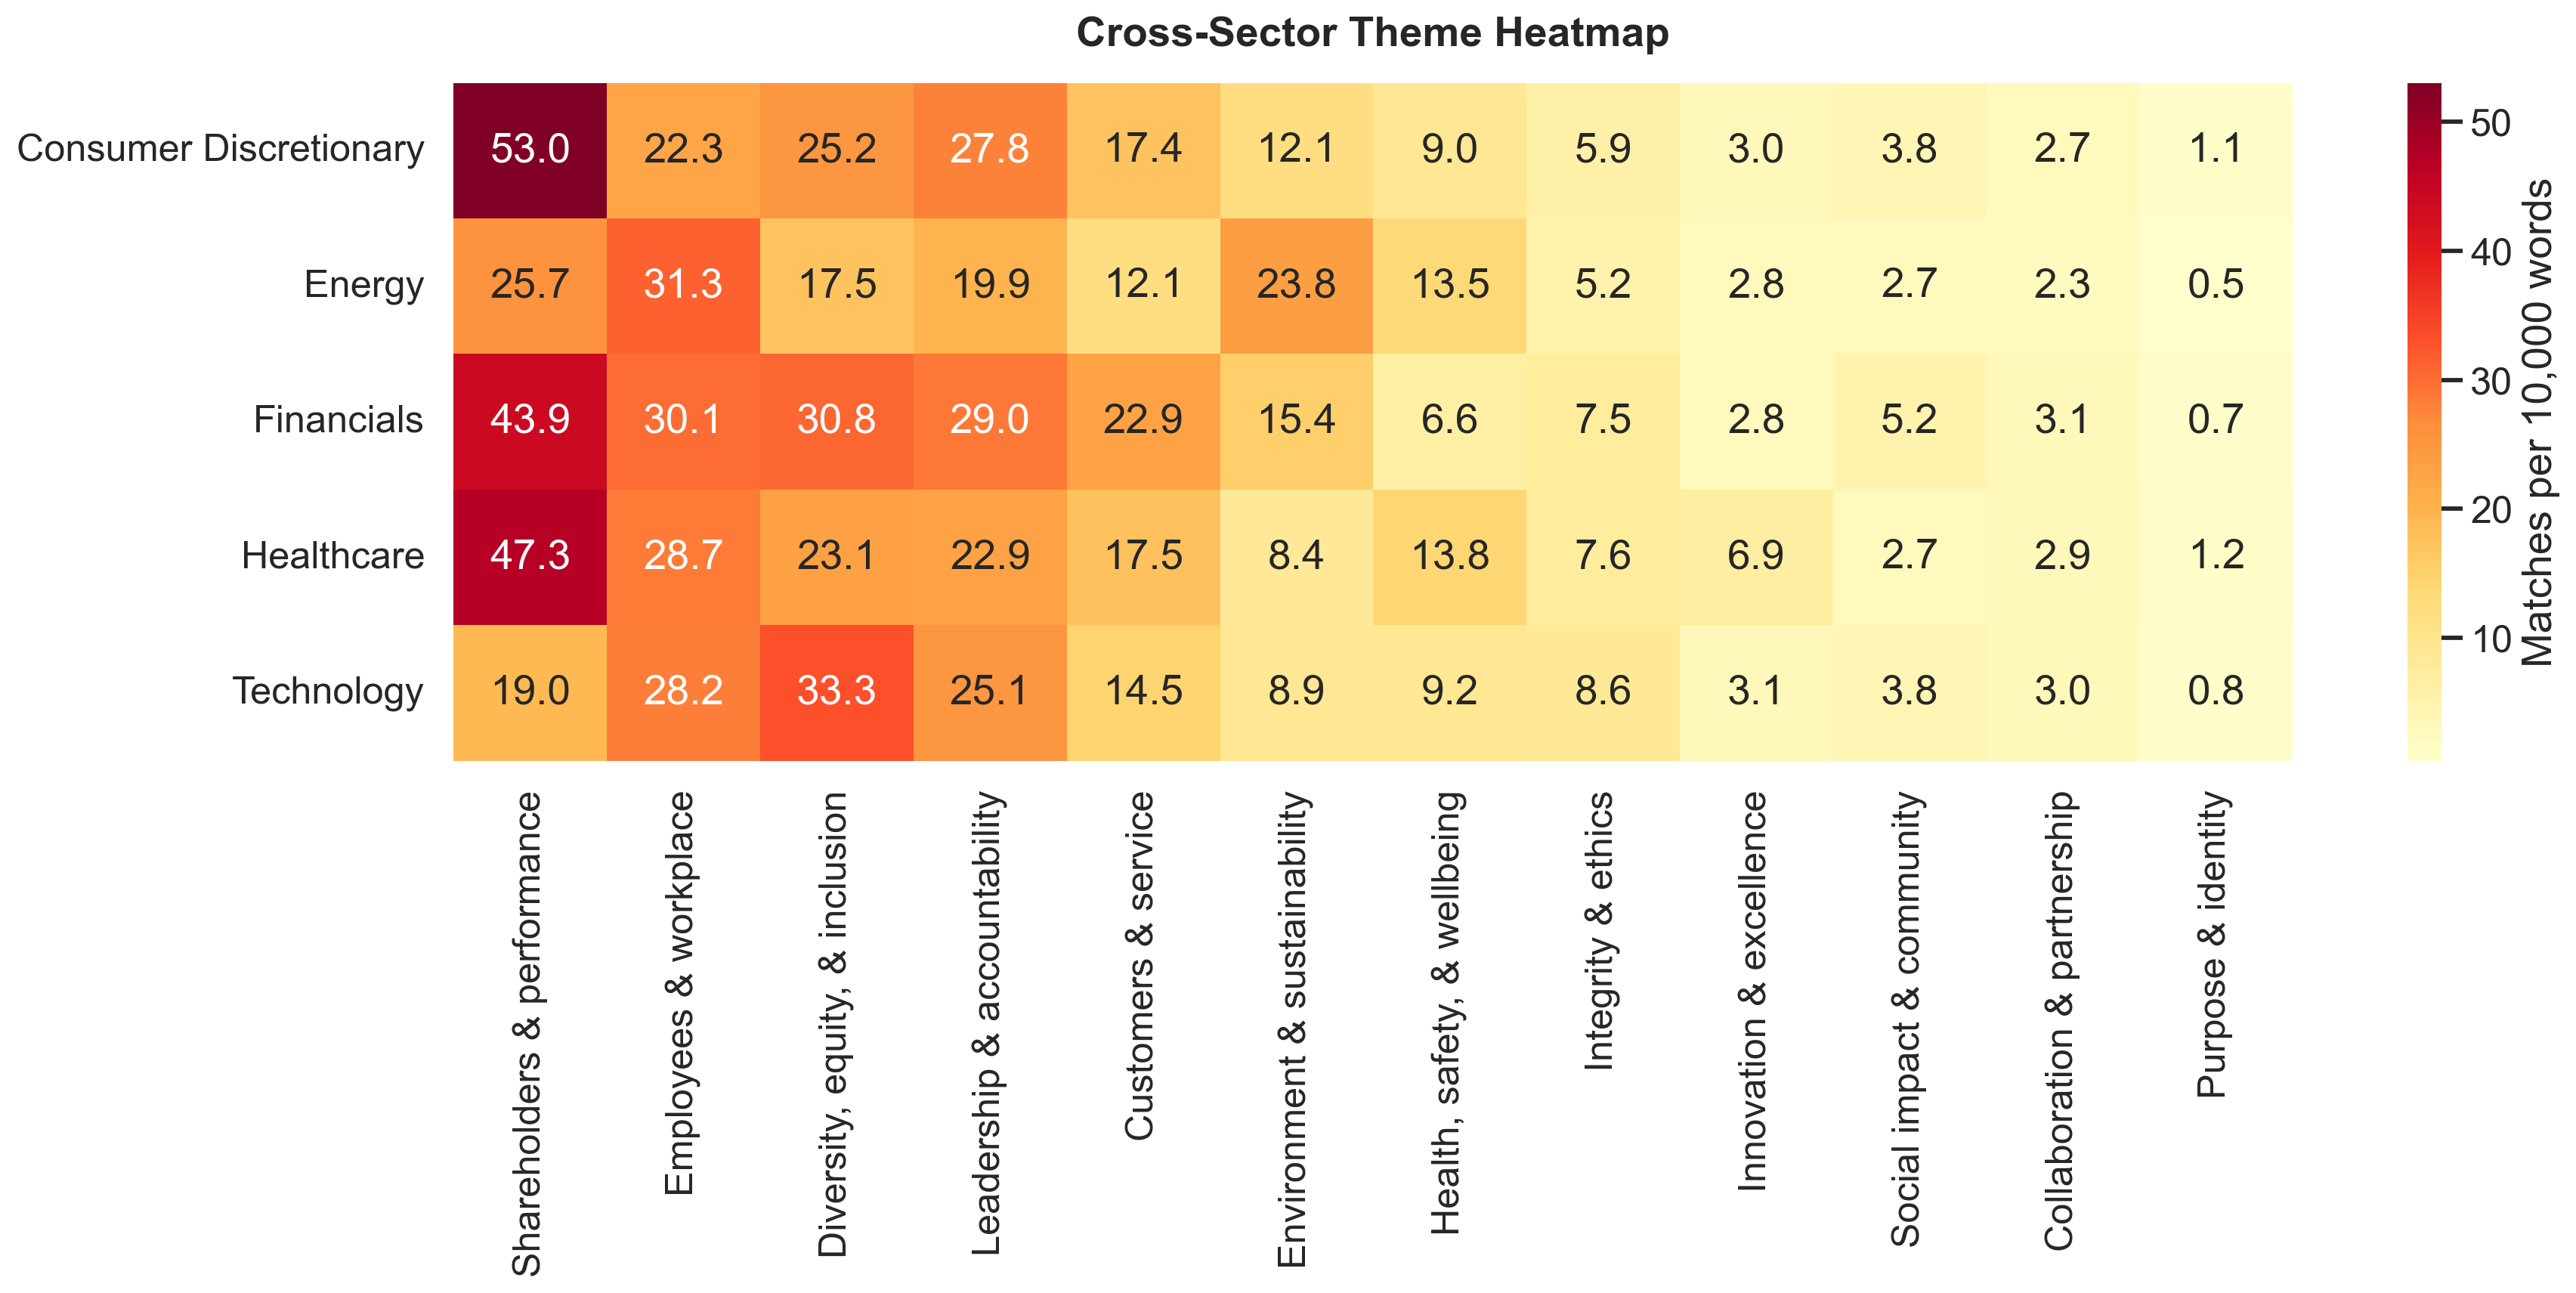
\includegraphics[width=0.74\linewidth]{part2_lived_values/outputs/text_mining/figures/sector_theme_heatmap.png}
\caption{Sector-theme heatmap for proxy-statement theme emphasis}
\label{fig:proxy-sector-theme}
\end{figure}

Figure \ref{fig:proxy-sector-theme} shows a common shareholder-governance backbone alongside
sector-specific vocabularies. The brightest cells are shareholder/performance in Consumer
Discretionary (53.0), Healthcare (47.3), and Financials (43.9); Technology is distinctive for DEI
(33.3), while Energy is high on employees/workplace (31.3) and environment/sustainability (23.8).
Alignment scores should therefore be read with attention to sector-specific disclosure language.

\begin{figure}[H]
\centering
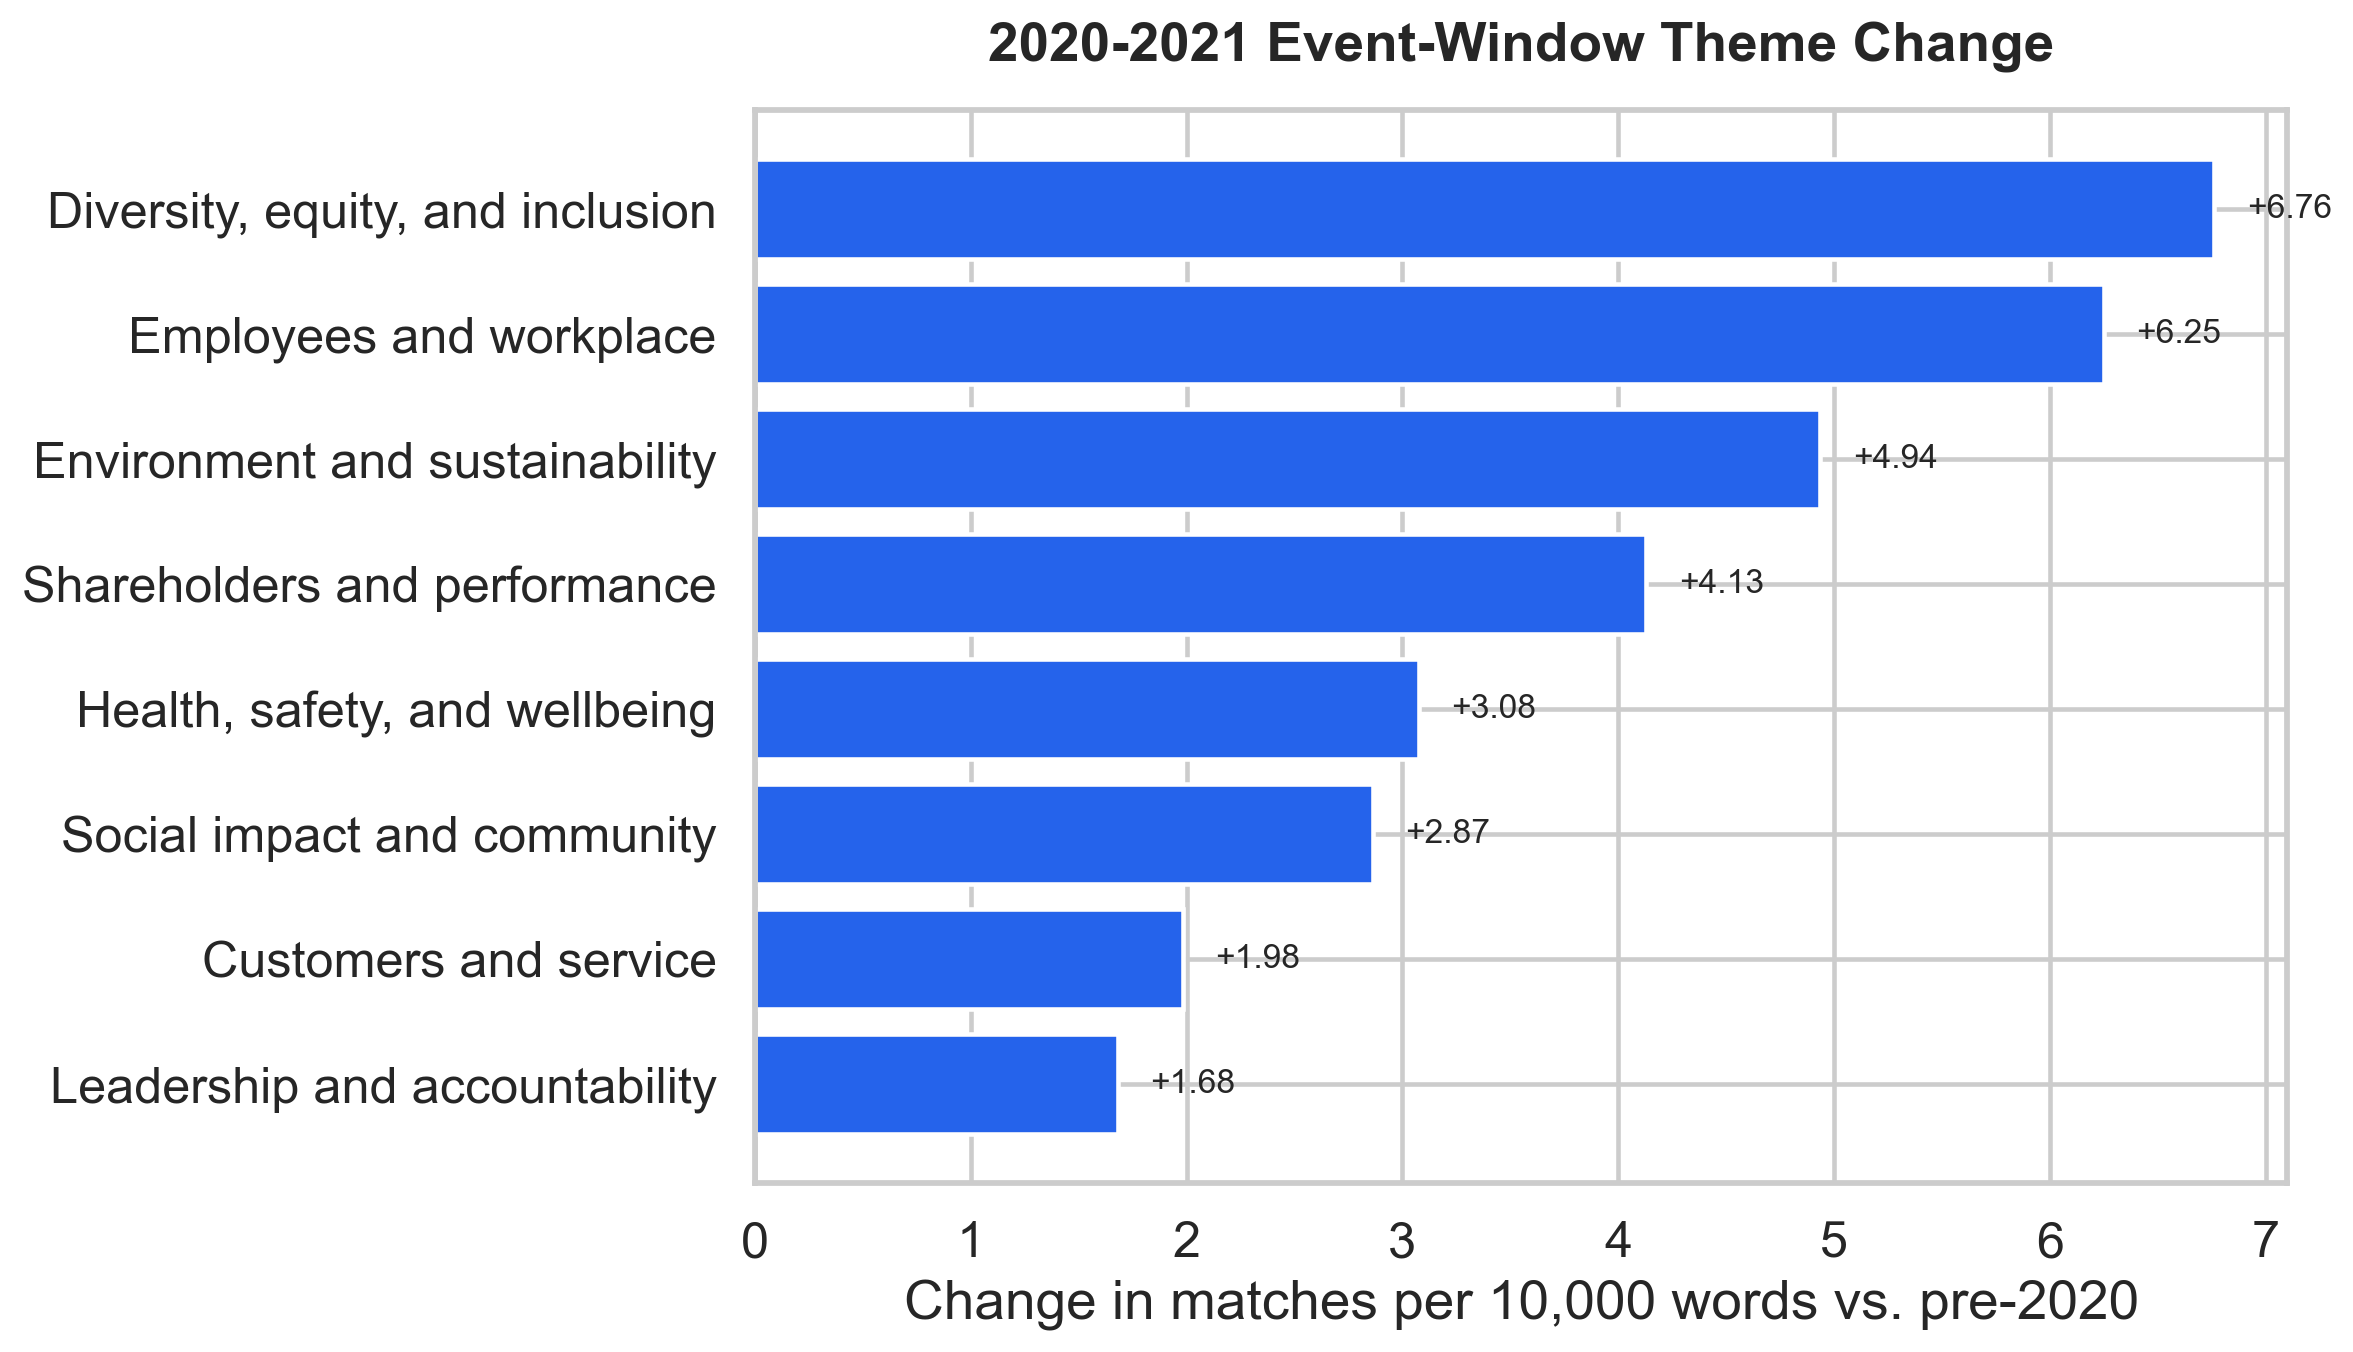
\includegraphics[width=0.66\linewidth]{part2_lived_values/outputs/text_mining/figures/event_window_theme_change.png}
\caption{Event-window change in proxy-statement theme emphasis}
\label{fig:proxy-event-window}
\end{figure}

Figure \ref{fig:proxy-event-window} shows the clearest descriptive increases around 2020--2021 for
DEI, employees and workplace, and health/safety language, consistent with a broader shift toward
workforce and stakeholder-facing disclosure. The figure is descriptive rather than causal; it shows
that the proxy corpus changed in ways the authenticity index must accommodate.

\subsection{Authenticity-index distribution}

Across 328 scored company-years, the mean authenticity index is 41.98 and the median is 44.83.
Scores range from 0.00 to 82.12, with an interquartile range of 30.81--55.14. The typical
company-year therefore shows moderate rather than high alignment: for the median row, less than
half of stated-values theme emphasis is mirrored in proxy-disclosure theme distribution.

\begin{figure}[H]
\centering
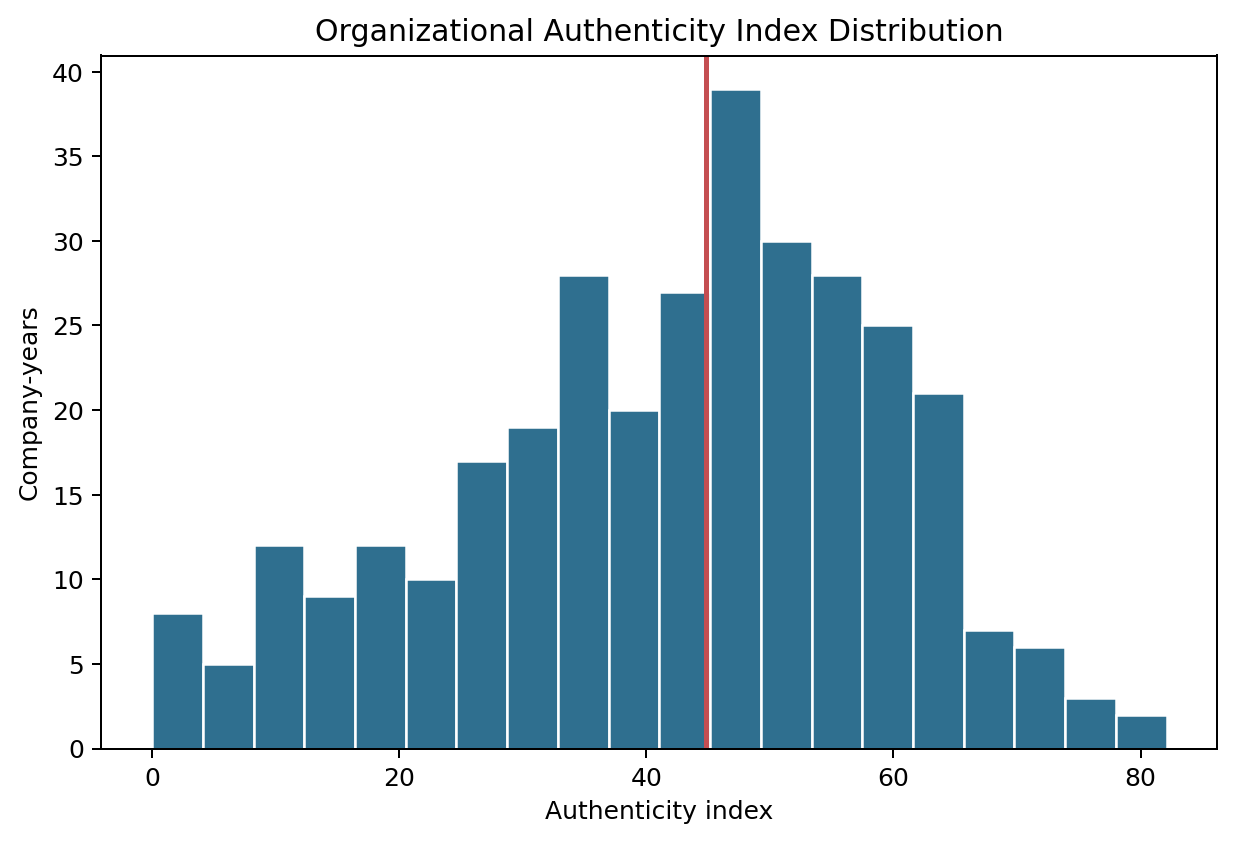
\includegraphics[width=0.60\linewidth]{part3_authenticity/outputs/figures/score_distribution.png}
\caption{Distribution of the authenticity index}
\label{fig:score-dist}
\end{figure}

Figure \ref{fig:score-dist} shows the core empirical distribution. Scores are not clustered near
either endpoint: the median company-year is moderately aligned, while a sizable lower tail signals
sharp divergence between stated values and proxy-disclosure priorities. This supports treating
authenticity as a graded alignment construct rather than a binary property.

\subsection{Sector and temporal patterns}

Sector averages vary descriptively. Energy and Healthcare have the highest average alignment scores
(47.03 and 46.74), while Consumer Discretionary and Financials are lower (36.31 and 37.08);
Technology sits near the overall mean at 42.58. These patterns should not be read as sector-level
behavioral authenticity because they may reflect sector vocabularies, reporting obligations,
document genre, and differential stated-values coverage.

\begin{table}[H]
\centering
\caption{Authenticity index by sector}
\label{tab:sector}
\begin{tabular}{lrrrr}
\toprule
Sector & Scored rows & Mean & Median & Range \\
\midrule
Consumer Discretionary & 59 & 36.31 & 41.99 & 0.51--64.49 \\
Energy & 62 & 47.03 & 46.03 & 1.57--82.12 \\
Financials & 74 & 37.08 & 37.58 & 0.60--72.50 \\
Healthcare & 73 & 46.74 & 49.97 & 6.27--72.76 \\
Technology & 60 & 42.58 & 45.16 & 0.00--66.09 \\
\bottomrule
\end{tabular}
\end{table}

Year summaries show modest upward movement after 2019, with average scores rising from 39.68 in
2016 to the low-to-mid 40s from 2019 through 2024. Because scored-row coverage also rises over
time, this descriptive pattern may partly reflect improved source availability rather than
substantive change.

\begin{figure}[H]
\centering
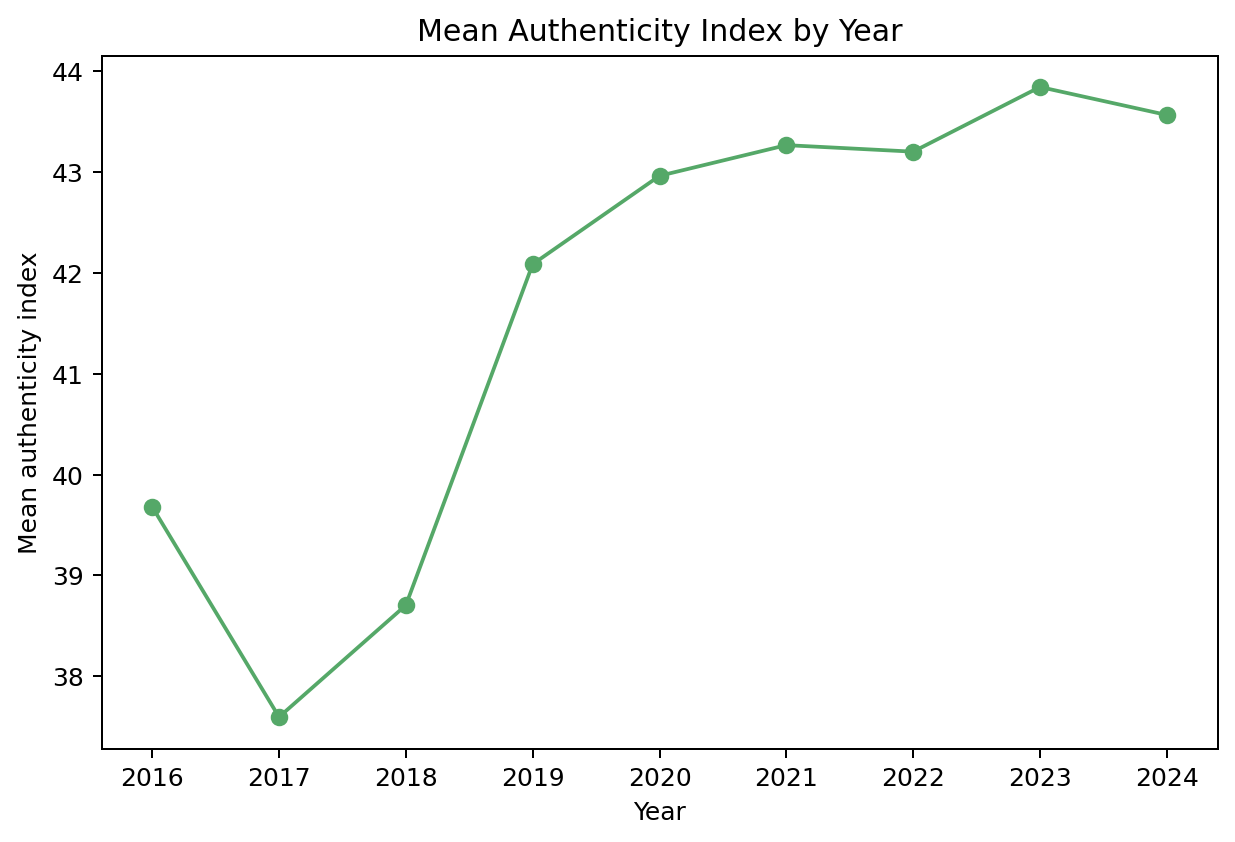
\includegraphics[width=0.58\linewidth]{part3_authenticity/outputs/figures/year_scores.png}
\caption{Mean authenticity index by year}
\label{fig:year}
\end{figure}

Figure \ref{fig:year} suggests a modest post-2019 increase, but later years also have better
stated-values coverage. The year pattern may therefore combine substantive change with improved
source availability.

\subsection{Robustness checks}

Table \ref{tab:robustness} summarizes robustness and diagnostic checks. The primary index is
strongly correlated with cosine alignment ($r=0.919$) and perfectly correlated with normalized L1
alignment by construction for probability distributions ($r=1.000$). Binary Jaccard overlap is
weaker ($r=0.778$), confirming that binary theme presence is less informative when proxy statements
mention many themes.

\begin{table}[H]
\centering
\caption{Robustness and diagnostic check summary}
\label{tab:robustness}
\begingroup
\footnotesize
\setlength{\tabcolsep}{2pt}
\renewcommand{\arraystretch}{1.12}
\begin{tabular}{>{\raggedright\arraybackslash}p{0.18\linewidth}
                >{\raggedright\arraybackslash}p{0.25\linewidth}
                >{\raggedright\arraybackslash}p{0.17\linewidth}
                >{\raggedright\arraybackslash}p{0.27\linewidth}}
\toprule
Check & Expected pattern & Observed result & Interpretation \\
\midrule
Cosine alignment & Strong positive association with the primary index. & Pearson $r=0.919$ & Theme-priority alignment is stable across distributional similarity metrics. \\
Normalized L1 alignment & Perfect or near-perfect association by construction for probability vectors. & Pearson $r=1.000$ & Confirms the overlap index is equivalent to common probability mass. \\
Binary Jaccard overlap & Positive but weaker association because it ignores emphasis intensity. & Pearson $r=0.778$ & Binary co-presence is informative but less precise than theme-share overlap. \\
Proxy word count & Weak association if length normalization works. & Pearson $r=-0.046$ & The index is not mechanically driven by proxy length. \\
Whole-text semantic score & Low-to-moderate association; embeddings may capture genre rather than values priorities. & Pearson $r=0.136$ for rows with semantic scores & Semantic similarity is useful as a contrast measure, not a substitute for the theme index. \\
\bottomrule
\end{tabular}
\endgroup
\end{table}

The near-zero proxy word-count correlation suggests that normalization removes mechanical length
effects. Whole-text semantic similarity is available for 342 rows and has low correlation with the
primary index among scored rows. This is useful: the embedding measure captures broad rhetorical or
genre similarity, whereas the primary index captures relative values-theme emphasis.

\begin{figure}[H]
\centering
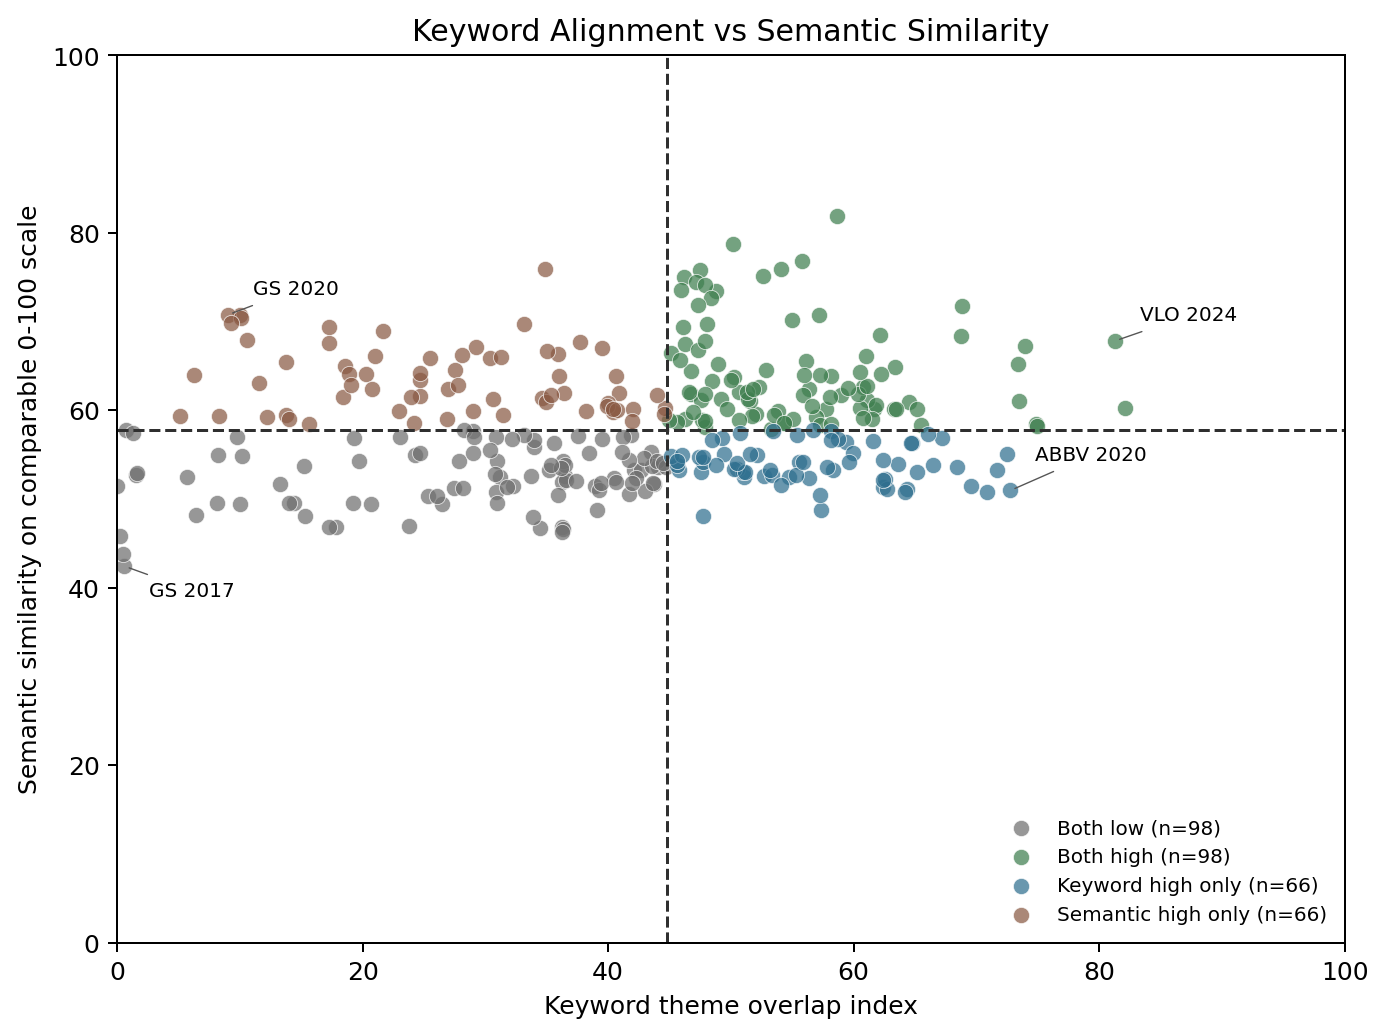
\includegraphics[width=0.62\linewidth]{part3_authenticity/outputs/figures/keyword_semantic_scatter.png}
\caption{Theme-distribution alignment versus semantic similarity}
\label{fig:keyword-semantic}
\end{figure}

Figure \ref{fig:keyword-semantic} shows why the semantic score is diagnostic rather than a
replacement for the index. The four quadrants identify keyword-semantic agreement or divergence;
the semantic-high-only quadrant is especially important because generic corporate or legal language
may mask theme-priority divergence.

\begin{figure}[H]
\centering
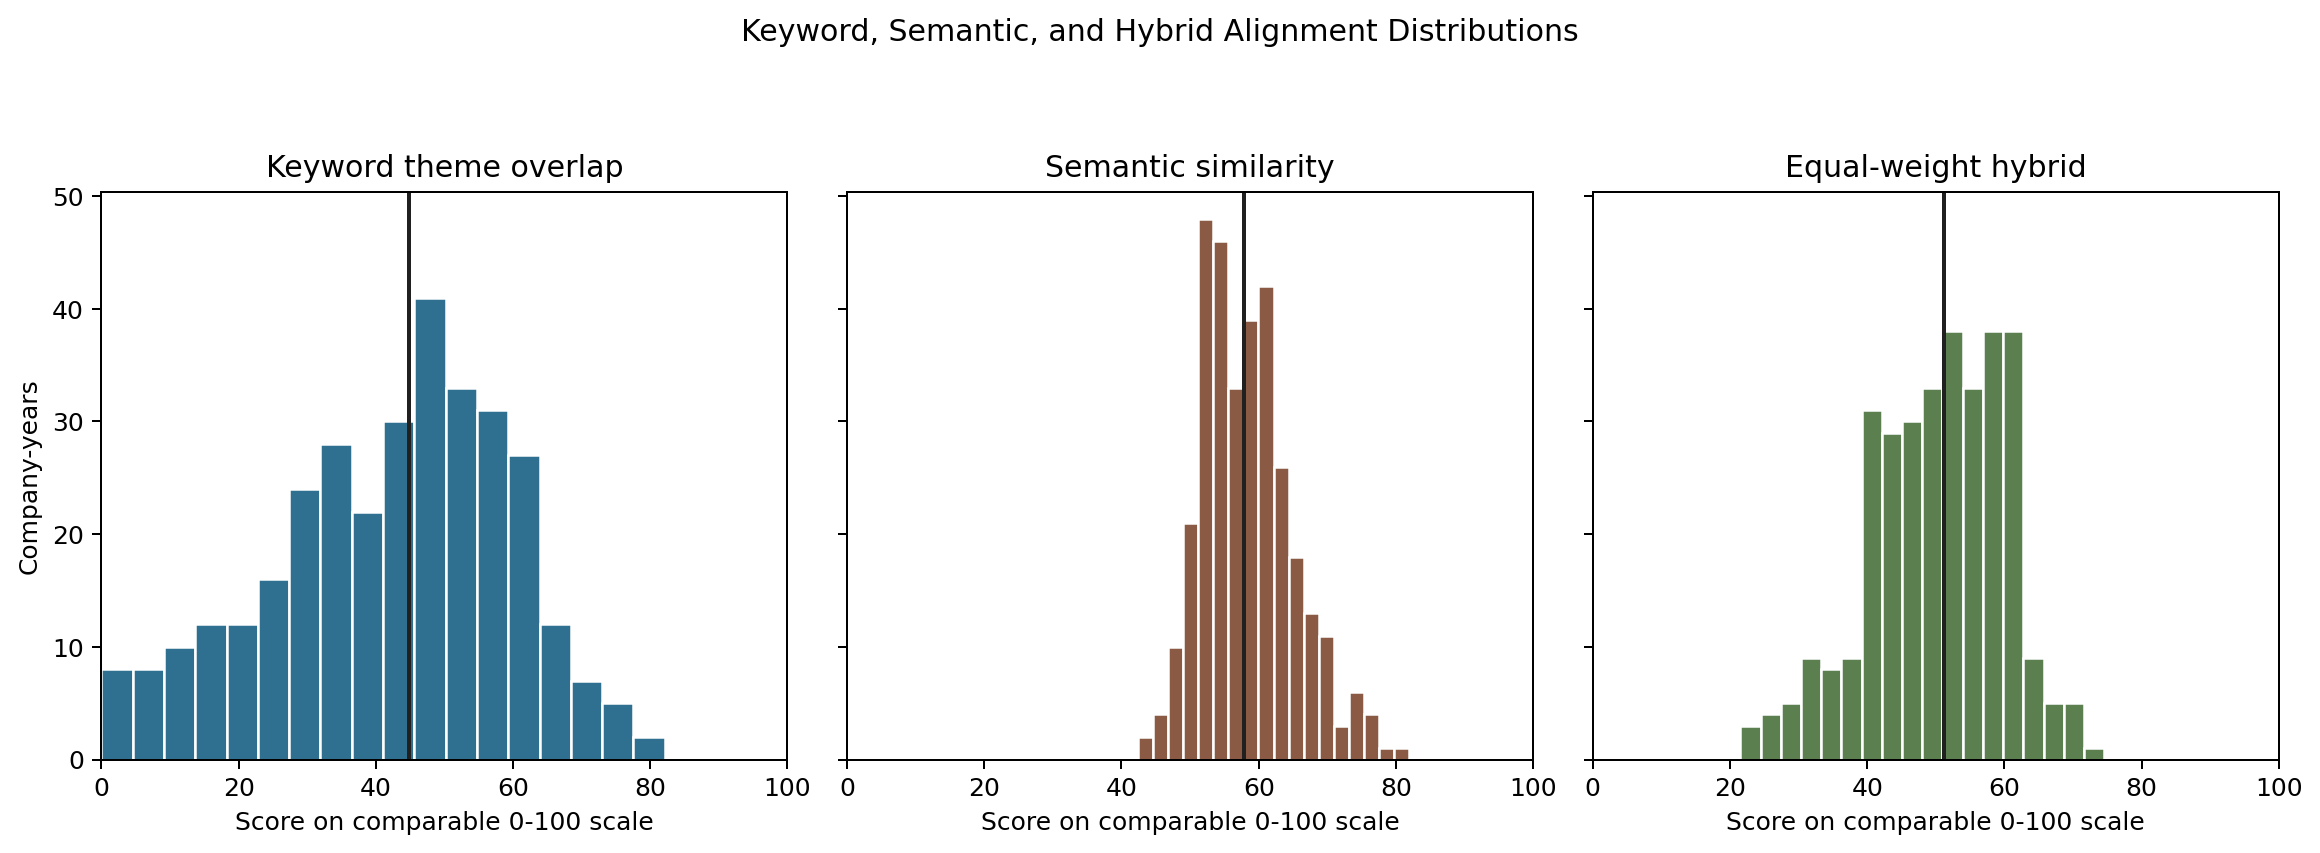
\includegraphics[width=0.86\linewidth]{part3_authenticity/outputs/figures/metric_comparison_distributions.png}
\caption{Distribution of robustness metrics}
\label{fig:metric-comparison}
\end{figure}

Figure \ref{fig:metric-comparison} compares keyword theme-overlap, whole-text semantic similarity,
and an equal-weight hybrid score. The semantic distribution is more compressed and centered higher
than the keyword index, while the hybrid falls between them. This supports keeping the keyword
index primary and using semantic similarity as a contrast diagnostic.

\section{Exploratory Measurement Diagnostics}

The diagnostic analysis asks whether proxy-statement genre and theme semantics affect the index. It
addresses three questions: (1) Is the index sensitive to whole-document proxy genre pressure? (2)
Which proxy sections carry values-theme evidence? (3) Are same-labeled themes semantically
comparable across stated-values pages and proxy statements?

\subsection{Proxy genre pressure}

Proxy genre pressure is computed from three phrase families: shareholder-meeting mechanics,
governance boilerplate, and legal/procedural language. Each count is normalized per 1,000 words,
z-scored, and averaged. Standardization prevents the most frequent phrase family from mechanically
dominating the composite while treating the three component rates as conceptually comparable.
Higher values indicate stronger procedural and governance-genre language. The composite is:

\begin{align}
\mathrm{GenrePressure}_{cy} &=
\frac{1}{3}\left[z(M_{cy}) + z(G_{cy}) + z(L_{cy})\right],
\end{align}

where $c$ indexes company and $y$ year. $M_{cy}$ is the shareholder-mechanics rate, $G_{cy}$ the
governance-boilerplate rate, and $L_{cy}$ the legal/procedural rate. Each component is phrase
matches per 1,000 proxy words, and $z(\cdot)$ standardizes among collected proxy rows. Proxy genre
pressure is weakly negatively correlated with the authenticity index: Pearson $r=-0.093$ and
Spearman $\rho=-0.141$. Mean authenticity is 44.19 in the low genre-pressure tercile and 39.70 in
the high tercile, a 4.48-point difference.

A descriptive fixed-effects regression with proxy word count, sector indicators, and year
indicators yields a proxy-genre-pressure coefficient of $-2.764$, with $R^2=0.096$. This is not a
causal estimate: controls absorb basic document scale, sector vocabulary, and period effects rather
than identify an exogenous genre shock. Genre pressure is therefore a modest measurement-risk signal,
not the main explanation for low scores.

\begin{figure}[H]
\centering
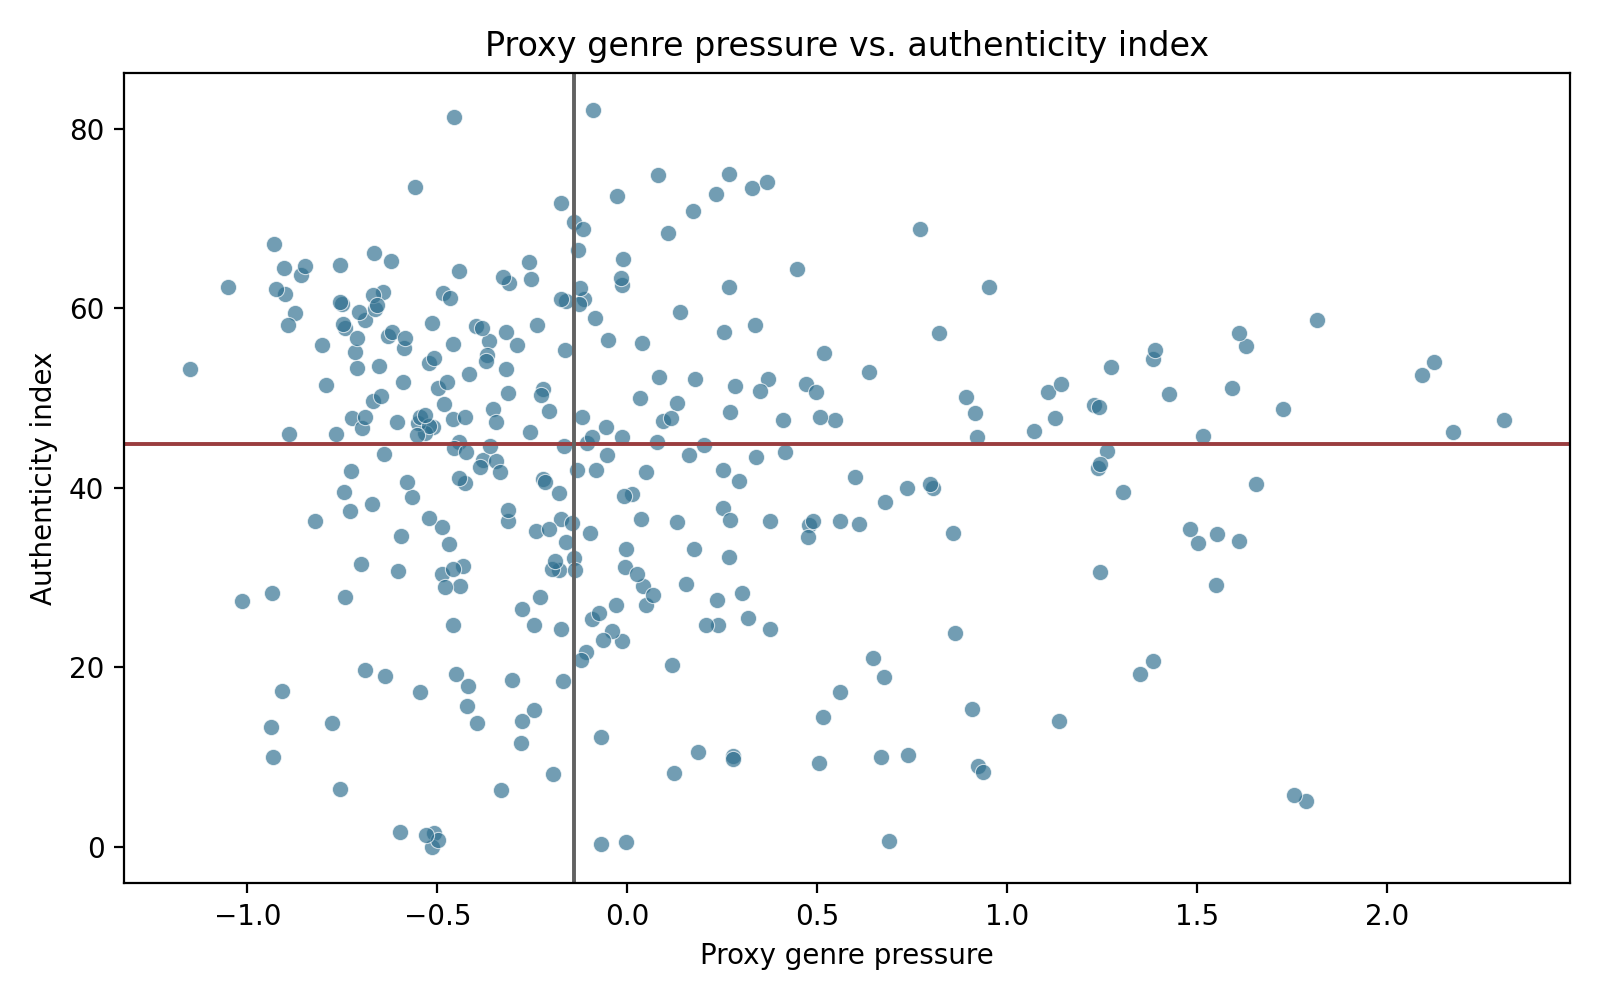
\includegraphics[width=0.62\linewidth]{part4_proposal/outputs/figures/genre_pressure_vs_authenticity.png}
\caption{Proxy genre pressure and authenticity}
\label{fig:genre-pressure}
\end{figure}

Figure \ref{fig:genre-pressure} shows diffuse scatter rather than a strong visual relationship,
matching the diagnostics: Pearson $r=-0.093$ is not conventionally significant ($p=0.093$), while
Spearman $\rho=-0.141$ is significant but small ($p=0.011$). Genre pressure is a modest measurement
concern, not the main explanation for low alignment.

\subsection{Section-level proxy parsing}

The section parser identifies 127,630 section-like spans across 434 collected proxy statements and
assigns them to governance/board, meeting/voting, compensation, shareholder proposals, ownership,
audit, legal/other, human-capital/values, and related families. This heuristic structural parser
uses headings and section cues to locate values language; it is not a legal-document parser. Its
construct-validity purpose is to distinguish evidence embedded in voting instructions or
table-of-contents fragments from evidence in governance, human-capital, compensation, and
sustainability contexts. Governance/board sections are the largest raw source, with 129,840 theme
matches; meeting/voting sections contribute 67,314, and human-capital/values sections 59,405.

Raw volume and density tell different stories. Governance/board sections dominate raw evidence
because they are large: 7,523,017 parsed words. Human-capital/values sections are most
values-dense, with 36.91 theme matches per 1,000 section words. Thus a theme match in a governance
section may carry a different textual meaning than the same match in a human-capital or values
section.

\begin{figure}[H]
\centering
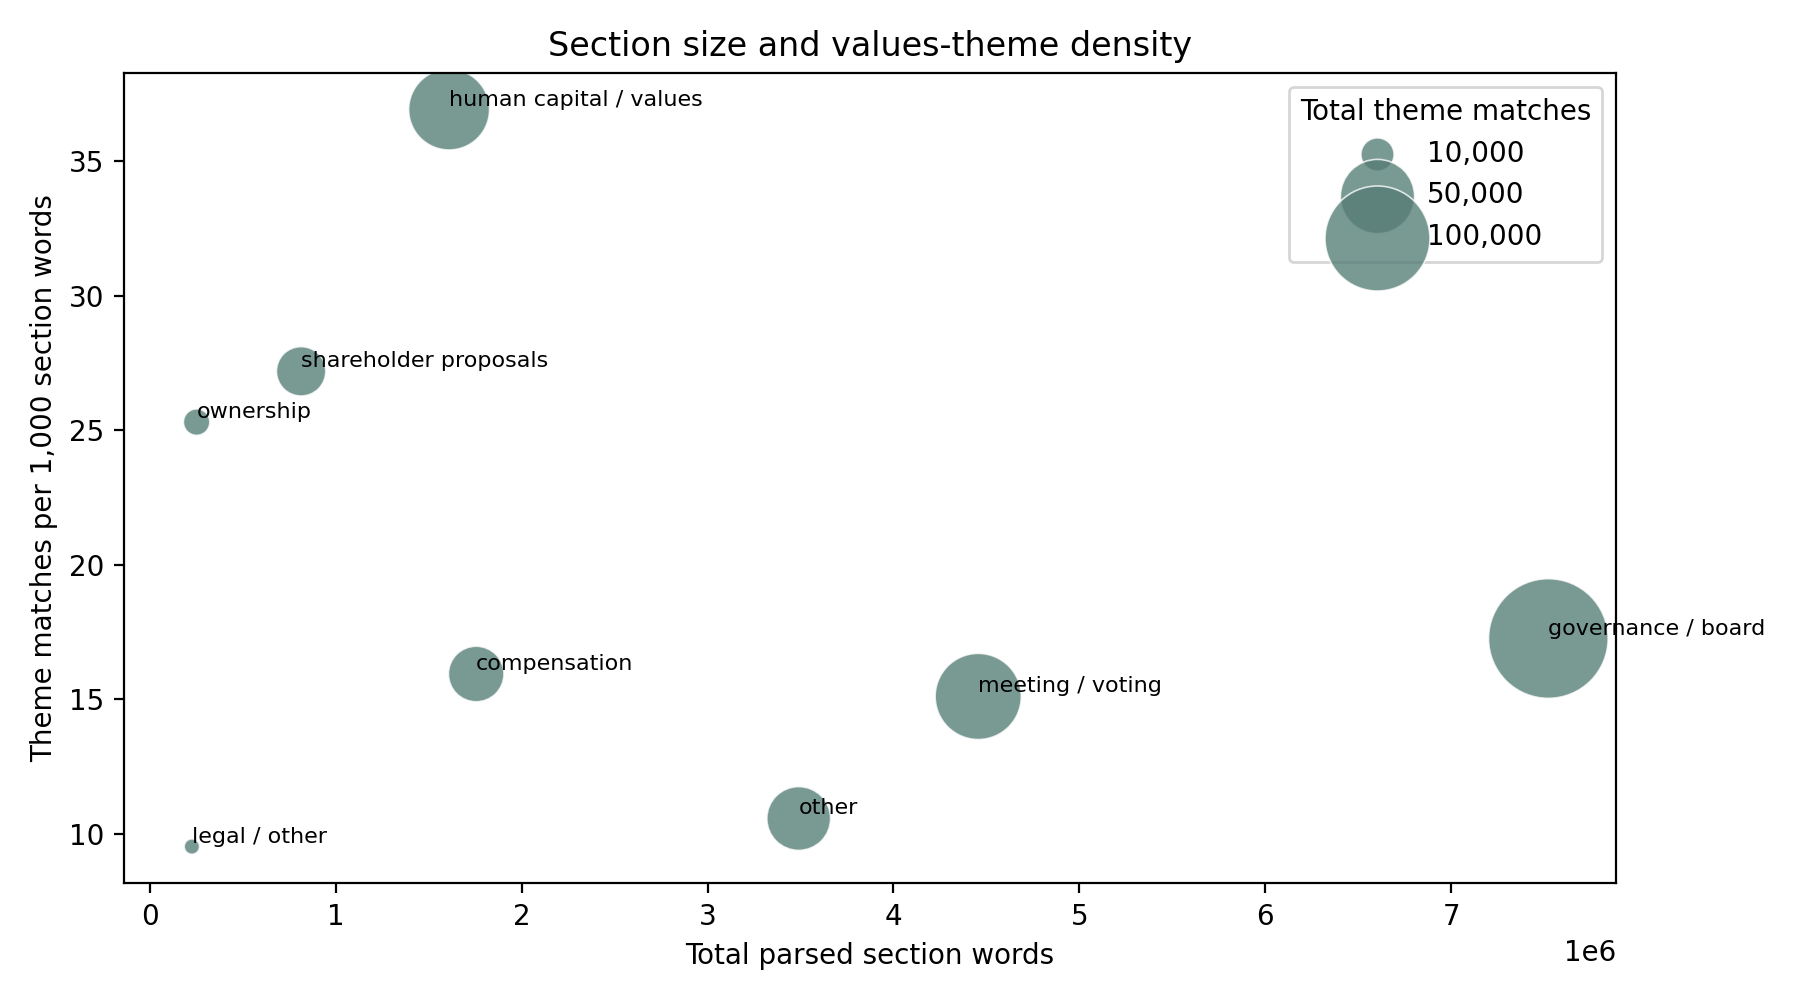
\includegraphics[width=0.70\linewidth]{part4_proposal/outputs/figures/section_theme_composition.png}
\caption{Section size and values-theme density}
\label{fig:section-bubble}
\end{figure}

Figure \ref{fig:section-bubble} visualizes the size-density distinction: the x-axis is total parsed
section volume, the y-axis values-theme density, and bubble size total theme matches.
Governance/board sections produce the largest raw volume, while human-capital/values sections are
far more values-dense. Raw counts alone would overstate governance machinery and understate direct
people-oriented values evidence.

\begin{figure}[H]
\centering
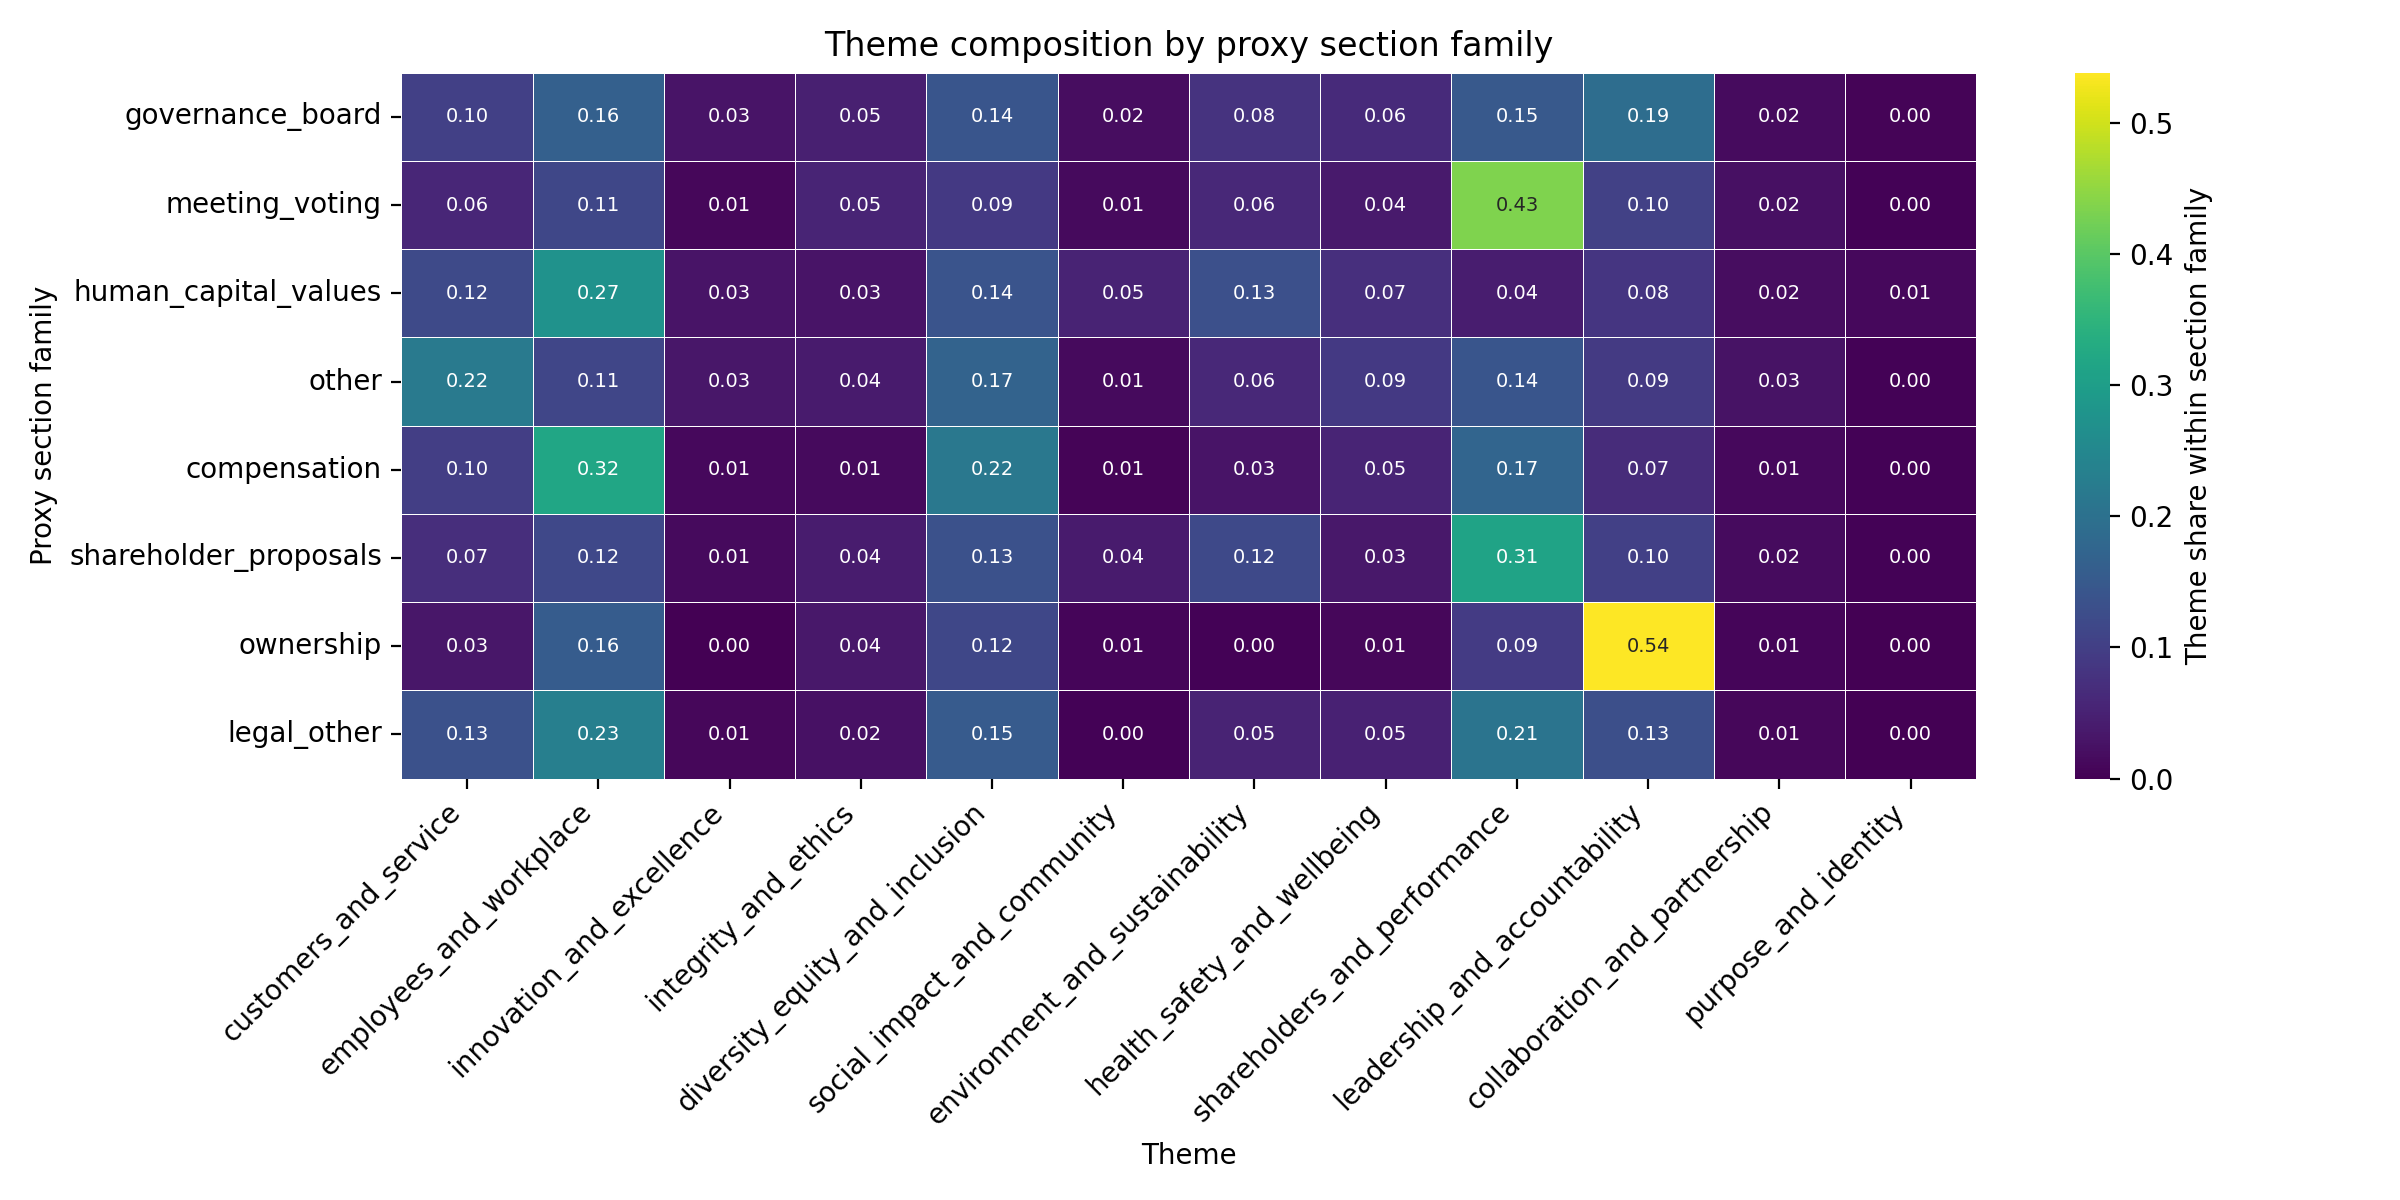
\includegraphics[width=0.76\linewidth]{part4_proposal/outputs/figures/section_theme_heatmap.png}
\caption{Theme composition by proxy section family}
\label{fig:section-heatmap}
\end{figure}

Figure \ref{fig:section-heatmap} should be read row-wise: each cell is a within-section-family
theme share, so brighter cells mark dominant themes within that family. The highlighted cells
separate proxy machinery from more direct values evidence: ownership sections concentrate on
leadership/accountability (0.54), meeting/voting and shareholder-proposal sections on
shareholder/performance (0.43 and 0.31), and compensation and human-capital/values sections on
employees/workplace (0.32 and 0.27).

\subsection{Theme-level semantic comparison}

The theme-level diagnostic compares stated-values and proxy-disclosure excerpts within the same
taxonomy theme. MiniLM semantic similarity is computed for 2,099 company-year-theme pairs where
both sides have evidence. This is stricter than whole-text semantic similarity because it asks
whether local language attached to the same theme label is similar. It addresses a dictionary
validity concern: two texts can match the same theme label while using it differently. For example,
``employees'' on a values page may refer to culture and belonging, while ``employees'' in a proxy
may appear in compensation or risk governance language.

Theme-level comparability varies sharply. Innovation and excellence has the highest mean local
semantic similarity (46.19), followed by environment and sustainability (45.83) and purpose and
identity (44.90). Employees and workplace is lowest (25.96), suggesting that stated-values pages
and proxy statements discuss employees in different local contexts: culture and people on the
stated-values side versus compensation, governance, workforce-risk, or human-capital disclosure in
proxy text. Customers and service has the largest mean stated/disclosure emphasis gap (0.167).

\begin{figure}[H]
\centering
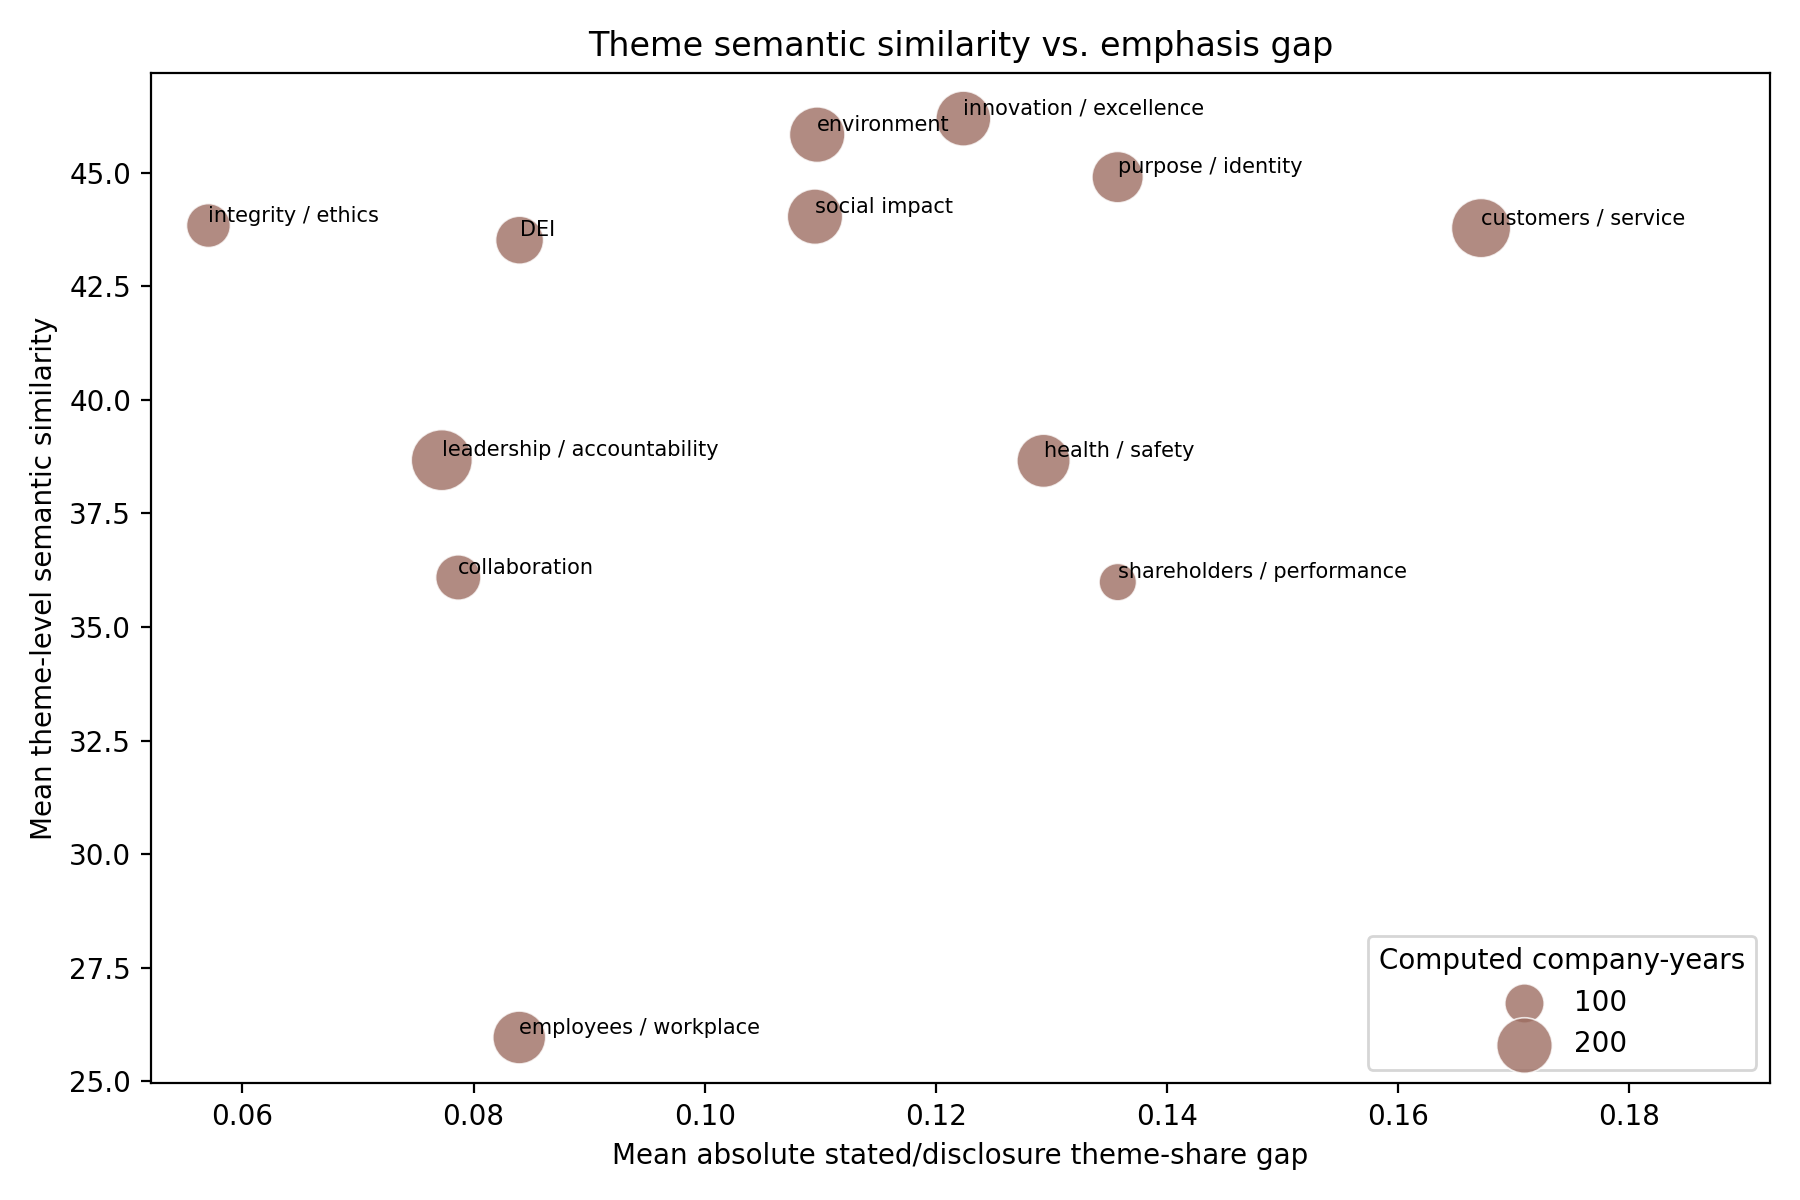
\includegraphics[width=0.68\linewidth]{part4_proposal/outputs/figures/theme_semantic_gap_scatter.png}
\caption{Theme semantic similarity and emphasis gap}
\label{fig:theme-semantic-gap}
\end{figure}

Figure \ref{fig:theme-semantic-gap} plots each taxonomy theme by its mean absolute stated/proxy
theme-share gap on the x-axis and mean local semantic similarity on the y-axis; bubble size is the
number of computed company-year-theme pairs. Customers/service has the largest emphasis gap despite
moderate semantic similarity, while employees/workplace is the clearest low-similarity outlier. The
figure shows why theme-level diagnostics add information beyond aggregate alignment.

\subsection{Illustrative case-audit targets}

The aggregate index is designed to produce audit targets rather than final judgments. Table
\ref{tab:case-audit} reports four illustrative company-years selected by the two primary diagnostic
dimensions: Organizational Authenticity Index (OAI) and whole-text semantic similarity (SS). Proxy
genre pressure (GP) is retained only as auxiliary context, not as a case-type criterion.

\begin{table}[H]
\centering
\scriptsize
\caption{Illustrative diagnostic case-audit targets}
\label{tab:case-audit}
\setlength{\tabcolsep}{3pt}
\renewcommand{\arraystretch}{1.12}
\begin{tabular}{l
                >{\raggedright\arraybackslash}p{0.17\linewidth}
                rrr
                >{\raggedright\arraybackslash}p{0.31\linewidth}}
\toprule
Case type & Company-year & OAI & SS & GP & Audit interpretation \\
\midrule
Low OAI, low SS & NVIDIA 2021 & 0.00 & 51.46 & -0.51 & Low alignment on both measures. \\
Low OAI, high SS & Goldman Sachs 2020 & 9.02 & 70.76 & 0.92 & Broad language similarity but weak theme alignment. \\
High OAI, low SS & AbbVie 2020 & 72.76 & 50.96 & 0.23 & Theme alignment with weaker whole-text similarity. \\
High OAI, high SS & Valero Energy 2024 & 81.28 & 67.81 & -0.46 & Robust alignment across both measures. \\
\bottomrule
\end{tabular}
\end{table}

This table is a triage device, not a qualitative validation exercise. The same index value should be
interpreted with diagnostic context. GP should be read after the OAI/SS pattern: higher GP may
indicate proxy mechanics diluting values evidence, while lower GP makes substantive stated/proxy
theme mismatch more plausible.

\section{Discussion}

The findings support three conclusions. First, large public firms show moderate, not high,
disclosure-priority alignment between stated-values pages and proxy statements. The mean
authenticity index is 41.98, the median is 44.83, and sector averages range from 36.31 in Consumer
Discretionary to 47.03 in Energy. These central results turn two public textual corpora into a
comparable company-year measure. Second, the index is not reducible to proxy boilerplate: proxy
genre pressure has a weak negative relationship with alignment but does not explain most variation.
Third, the source of values evidence matters. Proxy-side theme matches often arise in governance and
meeting machinery, while human-capital/values sections are more values-dense. Same theme labels are
not always semantically equivalent across source types; employees/workplace is common in both
sources but differs substantially in local meaning.

These results support interpreting the index as an audit tool. High scores indicate public-artifact
consistency across two communication channels. Low scores indicate divergence that may reflect true
differences in emphasis, source missingness, narrow stated-values pages, document-genre effects, or
taxonomy limitations. The diagnostics help distinguish these explanations.

\section{Limitations}

The most important limitation is construct validity. Proxy statements are official disclosure
documents, not direct observations of organizational behavior, so the index measures
disclosure-priority alignment rather than culture or ethical conduct. A second limitation is model
dependence: the deterministic taxonomy is auditable but can miss synonyms or context; semantic
checks help but do not solve this issue. Third, missingness is nonrandom because only 328 of 450
company-years can be scored. Fourth, the heuristic section parser can misclassify filing fragments,
especially when extracted proxy text contains table-of-contents artifacts or repeated headings.
Finally, all external-event interpretations are descriptive and should not be read causally.

\section{Conclusion}

This study demonstrates a scalable design for studying organizational authenticity as alignment
between stated values and official disclosure priorities. It collects historical stated-values
pages, pairs them with reproducible proxy disclosures, constructs an auditable theme-overlap index,
and stress-tests the index with semantic and genre diagnostics. The pipeline preserves the full
450 company-year sampling frame, documents missingness, and produces 328 scoreable observations,
making coverage part of the measurement object rather than an unreported preprocessing loss.

The main empirical result is moderate, not high, alignment. The mean Organizational Authenticity
Index is 41.98 on a 0--100 scale, with meaningful sector and year variation. Technology has the
highest sector mean, Consumer Discretionary the lowest, and average alignment rises after 2020. The
proxy corpus also contains substantive values evidence rather than only legal template language:
shareholder/performance themes dominate, but employee, DEI, leadership, environmental, and
stakeholder themes appear throughout the corpus and vary by sector and period.

The diagnostic evidence clarifies what the index should and should not be asked to do. Robustness
checks show that the index is not mechanically driven by proxy length or by whole-text semantic
similarity, and regression diagnostics indicate that proxy genre pressure is a modest measurement
risk rather than the main explanation for low scores. Section parsing shows that values language is
not evenly distributed across proxy statements: governance and meeting sections contain large
volumes of values-relevant language, while human-capital sections are smaller but more values-dense.
Theme-level semantic comparison further shows that some categories travel well across stated-values
pages and proxy disclosures, whereas employee/workplace language is especially context-dependent.

The resulting measure is therefore not a verdict on corporate authenticity, ethical behavior, or
organizational quality. It is a transparent instrument for identifying where public values claims and
official disclosure priorities align, diverge, or require qualitative review. Its strongest use is as
a reproducible screening and diagnostic tool: it can surface sector patterns, temporal shifts,
metric disagreements, and case-audit targets, while leaving final interpretation to contextual
reading and future validation against behavioral evidence.

\begin{thebibliography}{9}

\bibitem{hawn2016}
Hawn, O., and Ioannou, I. 2016. ``Mind the Gap: The Interplay Between External and Internal Actions
in the Case of Corporate Social Responsibility.'' \emph{Strategic Management Journal} 37(13):
2569--2588.

\bibitem{guiso2015}
Guiso, L., Sapienza, P., and Zingales, L. 2015. ``The Value of Corporate Culture.''
\emph{Journal of Financial Economics} 117(1): 60--76.

\bibitem{loughran2011}
Loughran, T., and McDonald, B. 2011. ``When Is a Liability Not a Liability? Textual Analysis,
Dictionaries, and 10-Ks.'' \emph{Journal of Finance} 66(1): 35--65.

\bibitem{meyerrowan1977}
Meyer, J. W., and Rowan, B. 1977. ``Institutionalized Organizations: Formal Structure as Myth and
Ceremony.'' \emph{American Journal of Sociology} 83(2): 340--363.

\bibitem{pamphile2023}
Pamphile, V. D., and Ruttan, R. L. 2023. ``The (Bounded) Role of Stated-Lived Value Congruence and
Authenticity in Employee Evaluations of Organizations.'' \emph{Organization Science} 34(6):
2332--2351.

\bibitem{reimers2019}
Reimers, N., and Gurevych, I. 2019. ``Sentence-BERT: Sentence Embeddings Using Siamese BERT-Networks.''
In \emph{Proceedings of the 2019 Conference on Empirical Methods in Natural Language Processing}.

\bibitem{shabana2016}
Shabana, K. M., and Ravlin, E. C. 2016. ``Corporate Social Responsibility Reporting as Substantive
and Symbolic Behavior: A Multilevel Theoretical Analysis.'' \emph{Business and Society Review}
121(2): 297--327.

\bibitem{wang2020}
Wang, W., Wei, F., Dong, L., Bao, H., Yang, N., and Zhou, M. 2020. ``MiniLM: Deep Self-Attention
Distillation for Task-Agnostic Compression of Pre-Trained Transformers.'' In \emph{Advances in
Neural Information Processing Systems}.

\end{thebibliography}

\end{document}
